\section{Eksperimenti}

Cilj ovog poglavlja je provesti eksperimentalnu evaluaciju razvijenog modela optimizacije raspodjele projektnih aktivnosti koji kombinira genetske algoritme (GA) i Monte Carlo simulaciju (MC).  
Eksperimenti će biti izvedeni prema unaprijed definiranom planu kako bi se dobili usporedivi i ponovljivi rezultati.

\subsection{Testni podaci}
Za potrebe eksperimenta koristit će se sintetički skupovi podataka generirani na temelju stvarnih distribucija trajanja aktivnosti i troškova resursa.  
Parametri uključuju:
\begin{itemize}
    \item Broj aktivnosti: 20--50.
    \item Vrijednosti aktivnosti (ROI) u rasponu 1000--10000 jedinica.
    \item Troškovi resursa proporcionalni složenosti aktivnosti.
    \item Varijabilna trajanja aktivnosti: optimistično ($t_o$), realno ($t_m$), pesimistično ($t_p$) prema PERT distribuciji.
\end{itemize}
Takav pristup omogućava kontrolu nad parametrima te usporedivost rezultata između različitih scenarija.

\subsection{Scenariji testiranja}
Eksperimenti će biti podijeljeni u tri osnovna scenarija:
\begin{enumerate}
    \item \textbf{Samo GA} — Genetski algoritam optimizira raspodjelu bez uključivanja Monte Carlo simulacije (baseline pristup).
    \item \textbf{Samo MC} — Monte Carlo simulacija koristi se za procjenu trajanja i uspješnosti bez GA optimizacije.
    \item \textbf{Kombinacija GA + MC} — Predloženi hibridni pristup gdje se GA koristi za optimizaciju, a MC za evaluaciju potencijalnih rješenja (finalni model).
\end{enumerate}

\subsection{Parametri eksperimenta}
Za sve scenarije koristit će se iste vrijednosti osnovnih parametara:
\begin{itemize}
    \item Veličina populacije (GA): 50, 100, 200.
    \item Broj generacija (GA): 50, 100.
    \item Broj Monte Carlo iteracija: 1000, 5000.
    \item Vjerojatnost križanja (GA): 0.8.
    \item Vjerojatnost mutacije (GA): 0.1.
\end{itemize}

\subsection{Kombinacije testova}
Planirane kombinacije eksperimenta prikazane su u Tablici \ref{tab:test_kombinacije}.

\begin{table}[H]
\centering
\caption{Planirane kombinacije eksperimenata}
\label{tab:test_kombinacije}
\begin{tabular}{|c|c|c|c|}
\hline
\textbf{Scenarij} & \textbf{Veličina populacije} & \textbf{Generacije} & \textbf{MC iteracije} \\ \hline
Samo GA & 50 / 100 / 200 & 50 / 100 & - \\ \hline
Samo MC & - & - & 1000 / 5000 \\ \hline
GA + MC & 50 / 100 / 200 & 50 / 100 & 1000 / 5000 \\ \hline
\end{tabular}
\end{table}

\subsection{Metodologija}
Za svaki scenarij provodit će se više ponavljanja (minimalno 10) kako bi se smanjio utjecaj slučajnih varijacija.  
Planirane metrike koje će se prikupljati:
\begin{itemize}
    \item \textbf{Broj uspješnih projekata} — koliko projekata je završilo unutar planiranog roka i budžeta.
    \item \textbf{Ukupna ROI vrijednost} — ukupni povrat investicije iz optimizirane raspodjele.
    \item \textbf{Stabilnost rješenja} — varijacija rezultata kroz ponavljanja eksperimenta.
    \item \textbf{Vrijeme izvršavanja} — prosječno trajanje izvođenja algoritma.
\end{itemize}

\subsection{Plan prezentacije rezultata}
Nakon provedbe eksperimenata, rezultati će biti prikazani:
\begin{itemize}
    \item tablicama (kvantitativni rezultati i usporedbe),
    \item grafovima (vizualizacija trendova i distribucija),
    \item opisnim analizama (interpretacija dobivenih rezultata).
\end{itemize}

Primjer vizualizacije usporedbe prosječne uspješnosti između triju scenarija prikazan je na slici \ref{fig:usporedba_roi}.

\begin{figure}[H]
    \centering
    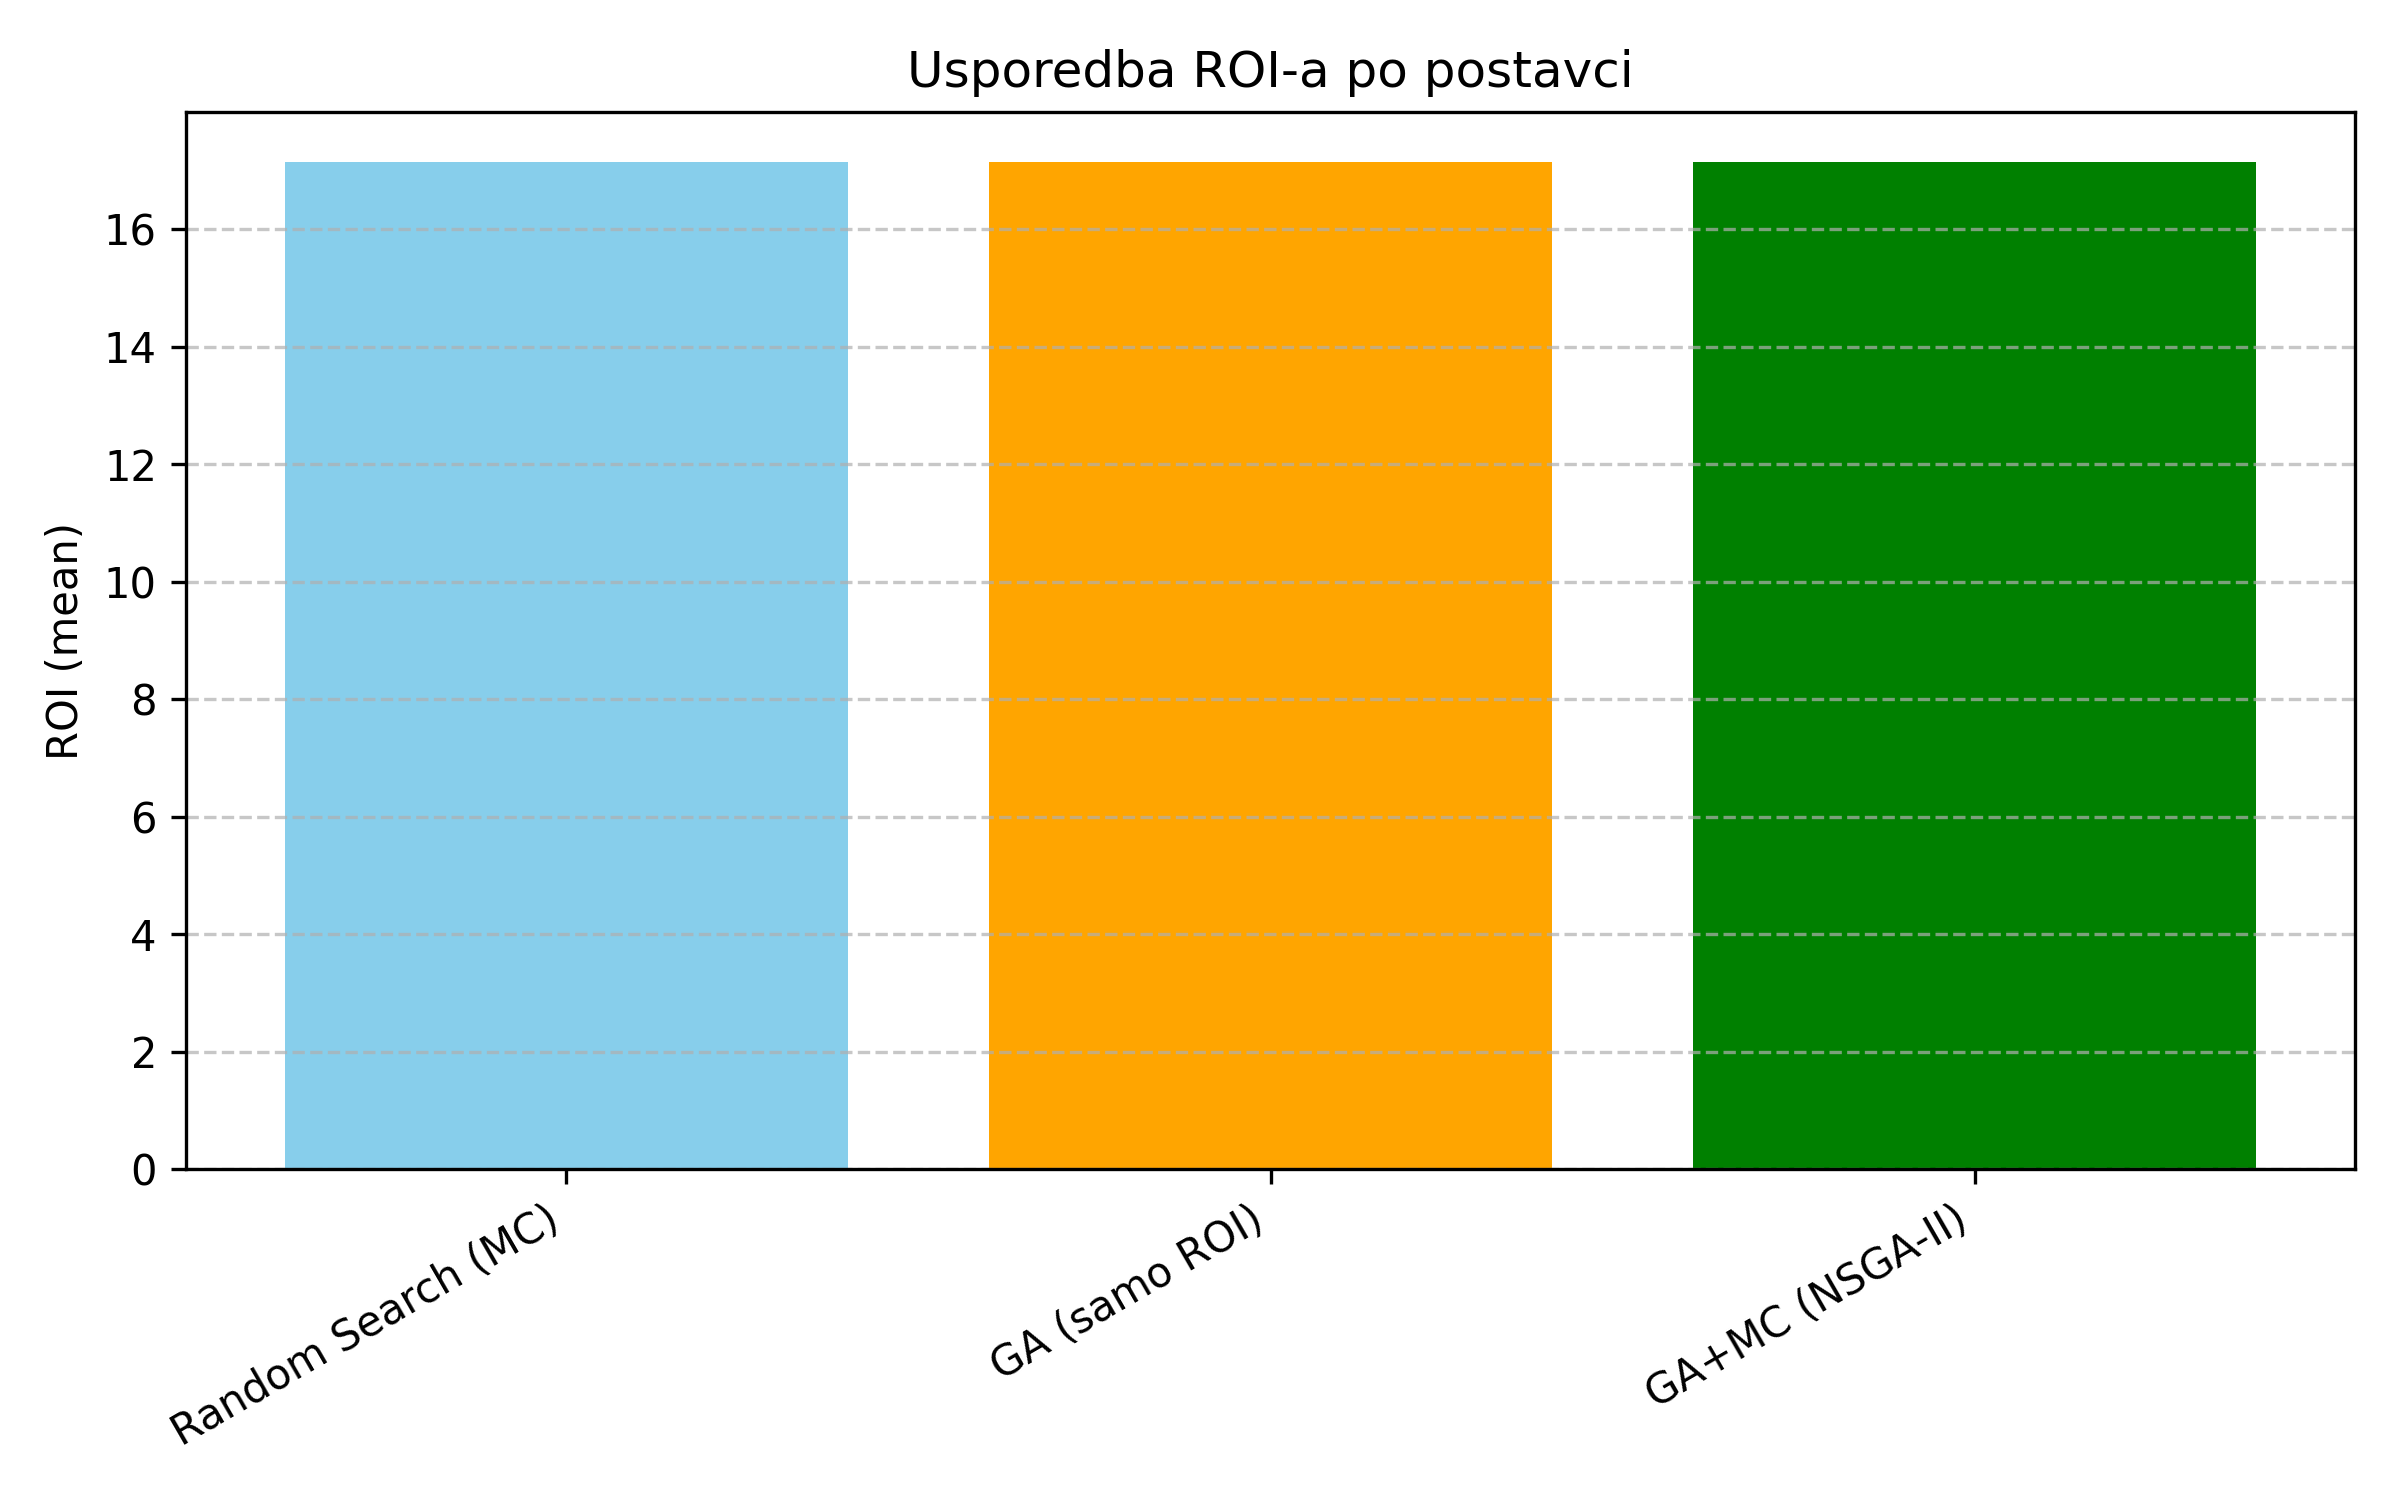
\includegraphics[width=0.85\textwidth]{slike/usporedba_roi.png}
    \caption{Primjer usporedbe prosječne uspješnosti za tri scenarija (primjer, podaci privremeni).}
    \label{fig:usporedba_roi}
\end{figure}
